\documentclass[14pt,a4paper,openbib]{extarticle}
\usepackage[utf8]{inputenc}
\usepackage[english,russian]{babel}
\usepackage{amsfonts,amssymb,amsmath}
\usepackage{amsthm}
\usepackage{latexsym}
\usepackage{cmap} % для кодировки шрифтов в pdf
\usepackage{mathtext}
\usepackage{indentfirst}
\usepackage{setspace}
%\usepackage{ulem}
\usepackage{enumerate}
\usepackage{graphics}
\usepackage[dvips]{graphicx}
\graphicspath{{images/}}
\pagestyle{plain}

\usepackage{listings} % Вменяемая поддержка листингов кода
\usepackage{xcolor} % Подстветка ^_^
\lstset{
    frame=tb, % draw a frame at the top and bottom of the code block
    tabsize=1, % tab space width
    showstringspaces=false, % don't mark spaces in strings
    numbers=left, % display line numbers on the left
    commentstyle=\color{green}, % comment color
    keywordstyle=\color{blue}, % keyword color
    stringstyle=\color{red} % string color
}

\newtheorem{opr}{Определение}[section] %Используется для автоматического нумерования определений
% Пример:
%\begin{opr}
%Функцией--оригиналом называется комплекснозначная\\ функция действительного переменного, удовлетворяющая следующим условиям
%\end{opr}

\numberwithin{equation}{section}
\usepackage[left=3cm, top=2cm, right=1.5cm, bottom=2cm, nohead]{geometry}
\linespread{1.3} % полуторный интервал
% Это плохой Times New Roman, который не умеет в жирный, курсив и черту :/
\renewcommand{\rmdefault}{ftm} % Times New Roman

\begin{document} % Начало документа
\begin{titlepage}
\begin{center}
МИНОБРНАУКИ РОССИИ

ФЕДЕРАЛЬНОЕ ГОСУДАРСТВЕННОЕ БЮДЖЕТНОЕ

ОБРАЗОВАТЕЛЬНОЕ УЧРЕЖДЕНИЕ

ВЫСШЕГО ОБРАЗОВАНИЯ

«ВОРОНЕЖСКИЙ ГОСУДАРСТВЕННЫЙ УНИВЕРСИТЕТ»

\begin{spacing}{4}
\end{spacing}

Математический факультет
\begin{spacing}{5.5}
\end{spacing}


Клиент-серверное приложение для управления персоналом и проектами
\begin{spacing}{4.5}
\end{spacing}


Выпускная квалификационная работа 

«Системный инженер (специалист по эксплуатации аппаратно-программных комплексов персональных ЭВМ и сетей на их основе)»

   \end{center}

   \begin{spacing}{5.5}
\end{spacing}

Допущено к защите в ИАК	 99.99.2019

\begin{spacing}{2}
\end{spacing}

\begin{spacing}{2}
\end{spacing}
Обучающийся \def\hrf#1{\hbox to#1{\hrulefill}}
\hrf{5em} А.А. Уткин
\begin{spacing}{2}
\end{spacing}
Руководитель\ \ \def\hrf#1{\hbox to#1{\hrulefill}}
\hrf{5em}
		 к.ф.-м.н., доц.	Груздев Д.В.

\begin{center}
\begin{spacing}{4}
\end{spacing}
Воронеж 2019
   \end{center}

\end{titlepage}
% Начало оглавления. Оно хитро заполняется само, глядя на заголовки
% которые добавляются с помощью \section и \subsection
\renewcommand\contentsname{Оглавление} %%% renaming the Table of Contents
\tableofcontents
\setcounter{page}{2}

\pagebreak
\section*{Введение}
% Такой заголовок пойдет в оглавление, только без нумерации
\addcontentsline{toc}{section}{Введение}
Программы для контроля процесса разработки очень популярны в наше время. Любой разработчик, а иногда и группа разработчиков, используют различные системы для контроля выполнения задач и проектов (например Gitlab issues или Redmine). В современном мире любая серьезная разработка продукта не может полноценно выполняться без подобных инструментов. Именно поэтому, для получения опыта разработки клиент-серверных приложений, было принято решение разработать систему управления персоналом и проектами.


\newpage
\section{Постановка задачи}
В процессе разработки была поставлена задача реализовать следующий функционал клиента:
\begin{enumerate} 
    \item Авторизация работника, смена пароля работником;
    \item Добавление и увольнение работников;
    \item Создание и завершение проектов;
    \item Назначение проектов работнику;
    \item Редактирование данных работников и проектов;
    \item Отображение назначенных работнику проектов;
    \item Отображения списка работников, назначенных на конкретный проект.
\end{enumerate}
Серверная часть должна была выполнять запросы клиента, оперировать данными в БД, а также отвечать за аутентификацию пользователей в системе.


\newpage
\section{Используемые технологии}
«Клиент — сервер» – вычислительная или сетевая архитектура, в которой задания или сетевая нагрузка распределены между поставщиками услуг, называемыми серверами, и заказчиками услуг, называемыми клиентами. Фактически клиент и сервер – это программное обеспечение. Обычно эти программы расположены на разных вычислительных машинах и взаимодействуют между собой через вычислительную сеть посредством сетевых протоколов.

Протокол передачи данных – набор соглашений интерфейса логического уровня, которые определяют обмен данными между различными программами. Эти соглашения задают единообразный способ передачи сообщений и обработки ошибок при взаимодействии программного обеспечения разнесённой в пространстве аппаратуры, соединённой тем или иным интерфейсом. Для установления связи между клиентом и сервером происходит по протоколу HTTPS.

HTTPS – расширение протокола HTTP для поддержки шифрования в целях повышения безопасности. Данные в протоколе HTTPS передаются поверх криптографических протоколов SSL или TLS.

HTTP – протокол прикладного уровня передачи данных изначально — в виде гипертекстовых документов в формате «HTML».

Для реализации задуманных идей был разработан собственный API, с помощью которого происходит общение клиенткой части с сервером.

API – описание способов (набор классов, процедур, функций, структур или констант), которыми одна компьютерная программа может взаимодействовать с другой программой.

Данные между клиентом и сервером передаются POST-запросами в формате JSON.

POST – один из многих методов запроса, поддерживаемых HTTP протоколом, используемым во Всемирной паутине. Метод запроса POST предназначен для запроса, при котором веб-сервер принимает данные, заключённые в тело сообщения, для хранения. Он часто используется для загрузки файла или представления заполненной веб-формы.

JSON – текстовый формат обмена данными, основанный на JavaScript, как и многие другие текстовые форматы, он легко читается людьми.

Для передачи данных аутентификации на сервер используется технология JSON Web Token (JWT).

JSON Web Token (JWT) – это открытый стандарт (RFC 7519) для создания токенов доступа, основанный на формате JSON. Как правило, используется для передачи данных для аутентификации в клиент-серверных приложениях.

В силу личного опыта и удобства, в качестве основного языка программирования был выбран Python.

Python – высокоуровневый язык программирования общего назначения, ориентированный на повышение производительности разработчика и читаемости кода. Синтаксис ядра Python минималистичен. В то же время стандартная библиотека включает большой объём полезных функций. Python поддерживает структурное, объектно-ориентированное, функциональное, императивное и аспектно-ориентированное программирование. Основные архитектурные черты — динамическая типизация, автоматическое управление памятью, полная интроспекция, механизм обработки исключений, поддержка многопоточных вычислений, высокоуровневые структуры данных. Поддерживается разбиение программ на модули, которые, в свою очередь, могут объединяться в пакеты.

Для создания интерфейса клиента использовался PyQt5 в связке с конструктором интерфейса Qt designer. Такой выбор обусловлен кроссплатформенностью этого инструмента, большой базой компонентов и возможностью создания собственных, а также подробной документацией PyQt5.

PyQt – набор «привязок» графического фреймворка Qt для языка программирования Python, выполненный в виде расширения Python.

Qt Designer – кроссплатформенная свободная среда для разработки графических интерфейсов (GUI) программ, использующих библиотеку Qt.

Для хранения и обработки данных использован виртуальный сервер (VPS) со следующим окружением:
\begin{enumerate} 
    \item Сервер базы данных MongoDB;
    \item Nginx для работы API;
    \item Gunicorn в качестве WSGI сервера;
    \item Серверная часть существует в виде Docker контейнера.
\end{enumerate}
MongoDB – документно-ориентированная система управления базами данных (СУБД) с открытым исходным кодом, не требующая описания схемы таблиц. Классифицирована как NoSQL, использует JSON-подобные документы и схему базы данных.

Nginx – веб-сервер и почтовый прокси-сервер, работающий на IX-подобных операционных системах.

WSGI – стандарт взаимодействия между Python-программой, выполняющейся на стороне сервера, и самим веб-сервером.

Docker – программное обеспечение для автоматизации развёртывания и управления приложениями в средах с поддержкой контейнеризации. Позволяет «упаковать» приложение со всем его окружением и зависимостями в контейнер, который может быть перенесён на любую Linux-систему.


\newpage
\section{Этапы создания сервера}
\subsection{Создание и настройка сервера}
Для разработки и отладки клиент-серверной архитектуры можно было обойтись локальным сервером. Но, для доступности из любого места и для реального видения скорости обработки данных, был арендован VPS сервер на территории России.

VPS – услуга предоставления в аренду так называемого виртуального выделенного сервера. В плане управления операционной системой по большей части она соответствует физическому выделенному серверу. В частности: root-доступ, собственные IP-адреса, порты, правила фильтрования и таблицы маршрутизации.

В качестве ОС VPS сервера была выбрана Ubuntu 18.04 LTS с базовой настройкой доступа и безопасности. После этого необходимо установить Docker, после чего устанавливается Docker-контейнер с собранным комплектом для работы MongoDB, Gunicorn и логики архитектуры. Так же необходим Docker-контейнер с настроенным Nginx. Все эти инструменты возможно установить и использовать без использования Docker, но в процессе разработки имели место частые смены VPS серверов.


\newpage
\subsection{Настройка работы HTTPS}
Для поддержки протокола передачи данных HTTPS, на сервере необходимо получить цифровой SSL сертификат.

Цифровой сертификат – выпущенный удостоверяющим центром электронный или печатный документ, подтверждающий принадлежность владельцу открытого ключа или каких-либо атрибутов. Сертификат открытого ключа удостоверяет принадлежность открытого ключа некоторому субъекту, например, пользователю. Сертификат открытого ключа содержит имя субъекта, открытый ключ, имя удостоверяющего центра, политику использования соответствующего удостоверяемому открытому ключу закрытого ключа и другие параметры, заверенные подписью удостоверяющего центра.

В данном случае, для шифрования трафика можно было обойтись самозаверенным сертификатом.

Самозаверенный сертификат — специальный тип сертификата, подписанный самим его субъектом. Технически данный тип ничем не отличается от сертификата, заверенного подписью удостоверяющего центра, только вместо передачи на подпись в удостоверяющий центр пользователь создаёт свою собственную сигнатуру. Создатель сертификата сам является в данном случае удостоверяющим центром.

Но, вместо создания самозаверенного сертификата было решено обратится к центру сертификации Let’s Encrypt.

Let’s Encrypt — центр сертификации, предоставляющий бесплатные криптографические сертификаты X.509 для TLS-шифрования (HTTPS). Процесс выдачи сертификатов полностью автоматизирован. Проект создан для того, чтобы большая часть интернет-сайтов смогла перейти к шифрованным подключениям (HTTPS). В отличие от коммерческих центров сертификации, в данном проекте не требуется оплата, переконфигурация веб-серверов, использование электронной почты, обработка просроченных сертификатов, что делает процесс установки и настройки TLS-шифрования значительно более простым.


\newpage
\subsection{Интеграция технологии JSON Web Token (JWT)}
Аутентификация пользователя происходит с помощью логина и пароля, после чего клиенту выдается токен для дальнейшего отправления данных. По истечению некоторого времени, этот токен необходимо обновить по средствам повторной аутентификации.

Токен представляет собой набор данных из трех секций в зашифрованном виде.
\begin{center}
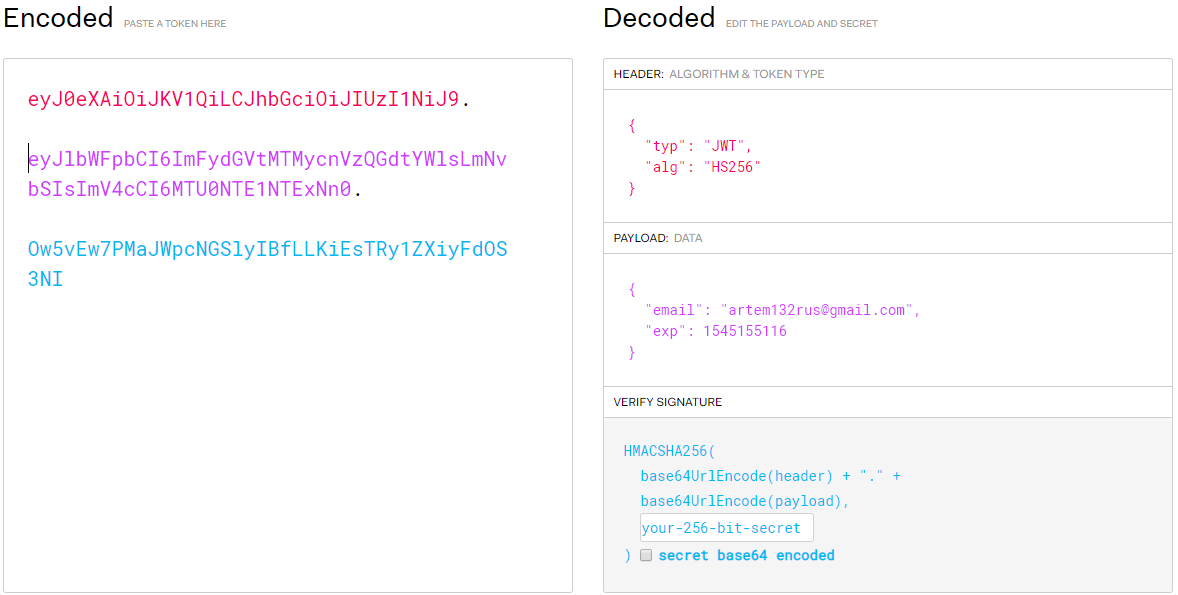
\includegraphics[width=\textwidth]{img/token1.png}\\
Рис. 1: структура токена.\\[\baselineskip]
% \\[\baselineskip] дает два перевода каретки, что пригодится далее
% Видимо, перевести каретку два раза ни разу не легко :/
\end{center}
Первая секция отвечает за информацию об используемых технологиях и шифровании. Во второй секции записан владелец токена (email), а также время, когда этот токен выдан. Третья секция содержит хеш-суммы первой и второй секции, для проверки токена на подлинность. Для безопасности, третья секция токена шифруется перед отправкой. Весь токен отправляется в кодировке Base64.

Base64 – стандарт кодирования двоичных данных при помощи только 64 символов ASCII.


\newpage
\subsection{Разработка собственного API}
Для взаимодействия сервера и клиента было разработано API, которое удовлетворяло всем нуждам. Созданное API позволяет передавать данные по средствам POST-запроса в формате JSON. Для оптимизации передачи данных, была добавлена возможность объединять множественные запросы в один POST-запрос перед отправкой. Ответ от сервера так же приходит в формате JSON, а если запрос был множественным, ответ на него будет содержать вложенные данные для ответа на каждый запрос.
\begin{center}
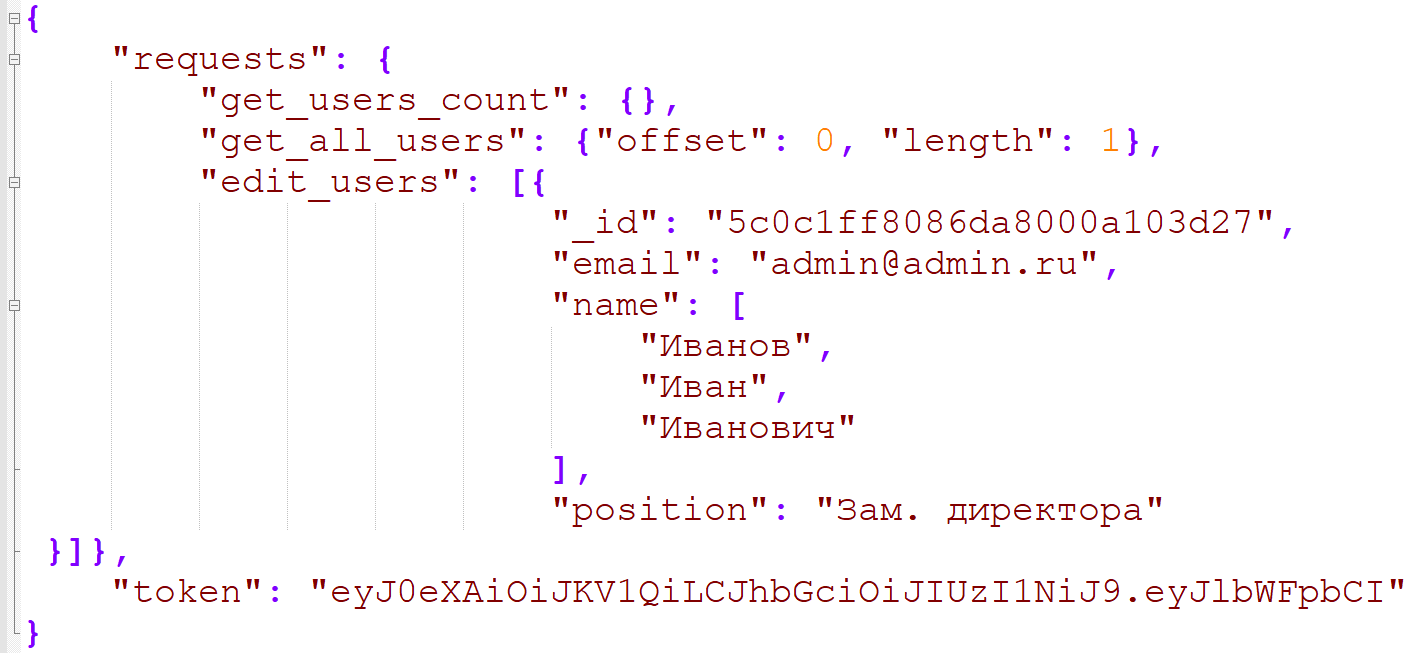
\includegraphics[width=\textwidth]{img/req.png}\\
Рис. 2: формат запроса к API. В данном случае, выполняется запрос на получение количества пользователей, получения данных одного из них, а также последующие редактирование этого пользователя.\\[\baselineskip]
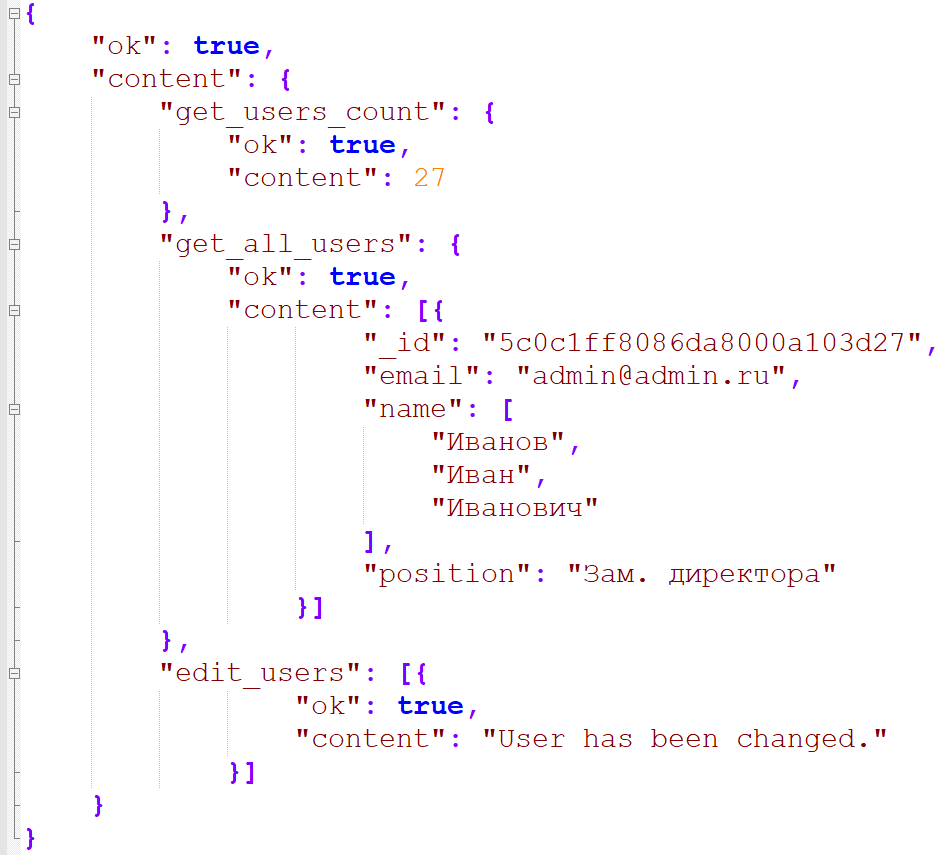
\includegraphics[scale=0.5]{img/ans.png}\\
Рис. 3: ответ сервера на запрос, представленный на рис. 2. Данные для каждого запроса были объединены в один JSON файл.\\[\baselineskip]
\end{center}


\newpage
\subsection{Реализация}
Основная логика работы с БД и обработки запросов реализована за счет языка программирования Python. Для обращения к БД (чтение, запись) используется библиотека pymongo. Для интеграции технологии JSON Web Token (JWT) используется библиотека jwt. Для обработки json файлов используется библиотека json.

Каждое логическое действие представляет собой обособленную функцию, которая будет вызвана при необходимости.
\begin{center}
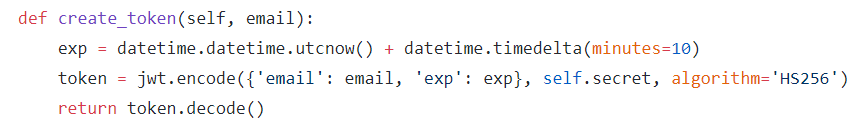
\includegraphics[width=\textwidth]{img/create_token.png}\\
Рис. 4: пример функции создания токена для клиента, прошедшего аутентификацию.\\[\baselineskip]
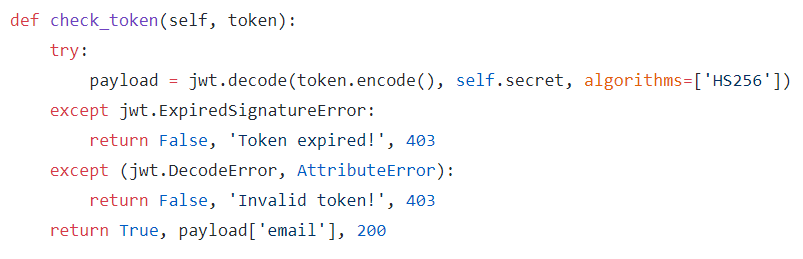
\includegraphics[scale=0.6]{img/check_token.png}\\
Рис. 5: пример функции проверки токена клиента.\\[\baselineskip]
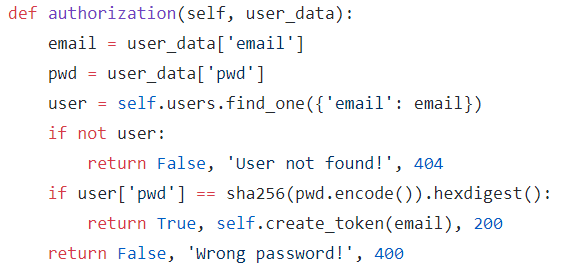
\includegraphics[scale=0.6]{img/authorization.png}\\
Рис. 6: пример функции авторизации клиента.\\[\baselineskip]
\end{center}

При взаимодействии с сервером используются коды состояния HTTP для сообщения о статусе различных операций.

Код состояния HTTP — часть первой строки ответа сервера при запросах по протоколу HTTP (HTTPS). Он представляет собой целое число из трёх десятичных цифр. Первая цифра указывает на класс состояния. За кодом ответа обычно следует отделённая пробелом поясняющая фраза на английском языке, которая разъясняет человеку причину именно такого ответа.

Примерами таких кодов могут быть:
\begin{itemize}
  \item 200 OK («хорошо»);
  \item 400 Bad Request («плохой, неверный запрос»);
  \item 404 Not Found («не найдено»).
\end{itemize}

Для проверки всех модулей сервера были использованы unit-тесты, исходные коды которых содержатся в файле tests.py.

Юнит-тестирование — процесс в программировании, позволяющий проверить на корректность отдельные модули исходного кода программы, наборы из одного или более программных модулей вместе с соответствующими управляющими данными, процедурами использования и обработки. 

\newpage
\section{Этапы создания клиента}
\subsection{Создание и настройка сервера}
Разработка клиентской части происходила в ОС Windows 10, где и решено было установить данные инструменты.

Для установки языка программирования Python с официального сайта был взят установочный файл и запущен с правами администратора. Дальнейшая настройка не требовалась.

Установка PyQt5 возможна с помощью менеджера пакетов pip, который идет в комплекте с языком программирования Python. После этого настройка не требуется. Такие вспомогательные инструменты, как Qt Designer будут установлены автоматически.

pip — система управления пакетами, которая используется для установки и управления программными пакетами, написанными на языке программирования Python.


\newpage
\subsection{Создание интерфейса}
Для создания макета интерфейса клиента использовался инструмент Qt Designer, позволяющий сразу увидеть результаты работы, включив превью-режим. Qt Designer создает ui-файлы, которые возможно конвертировать в необходимый формат. В данном случае, конвертирование происходило в формат языка программирования Python.
\begin{center}
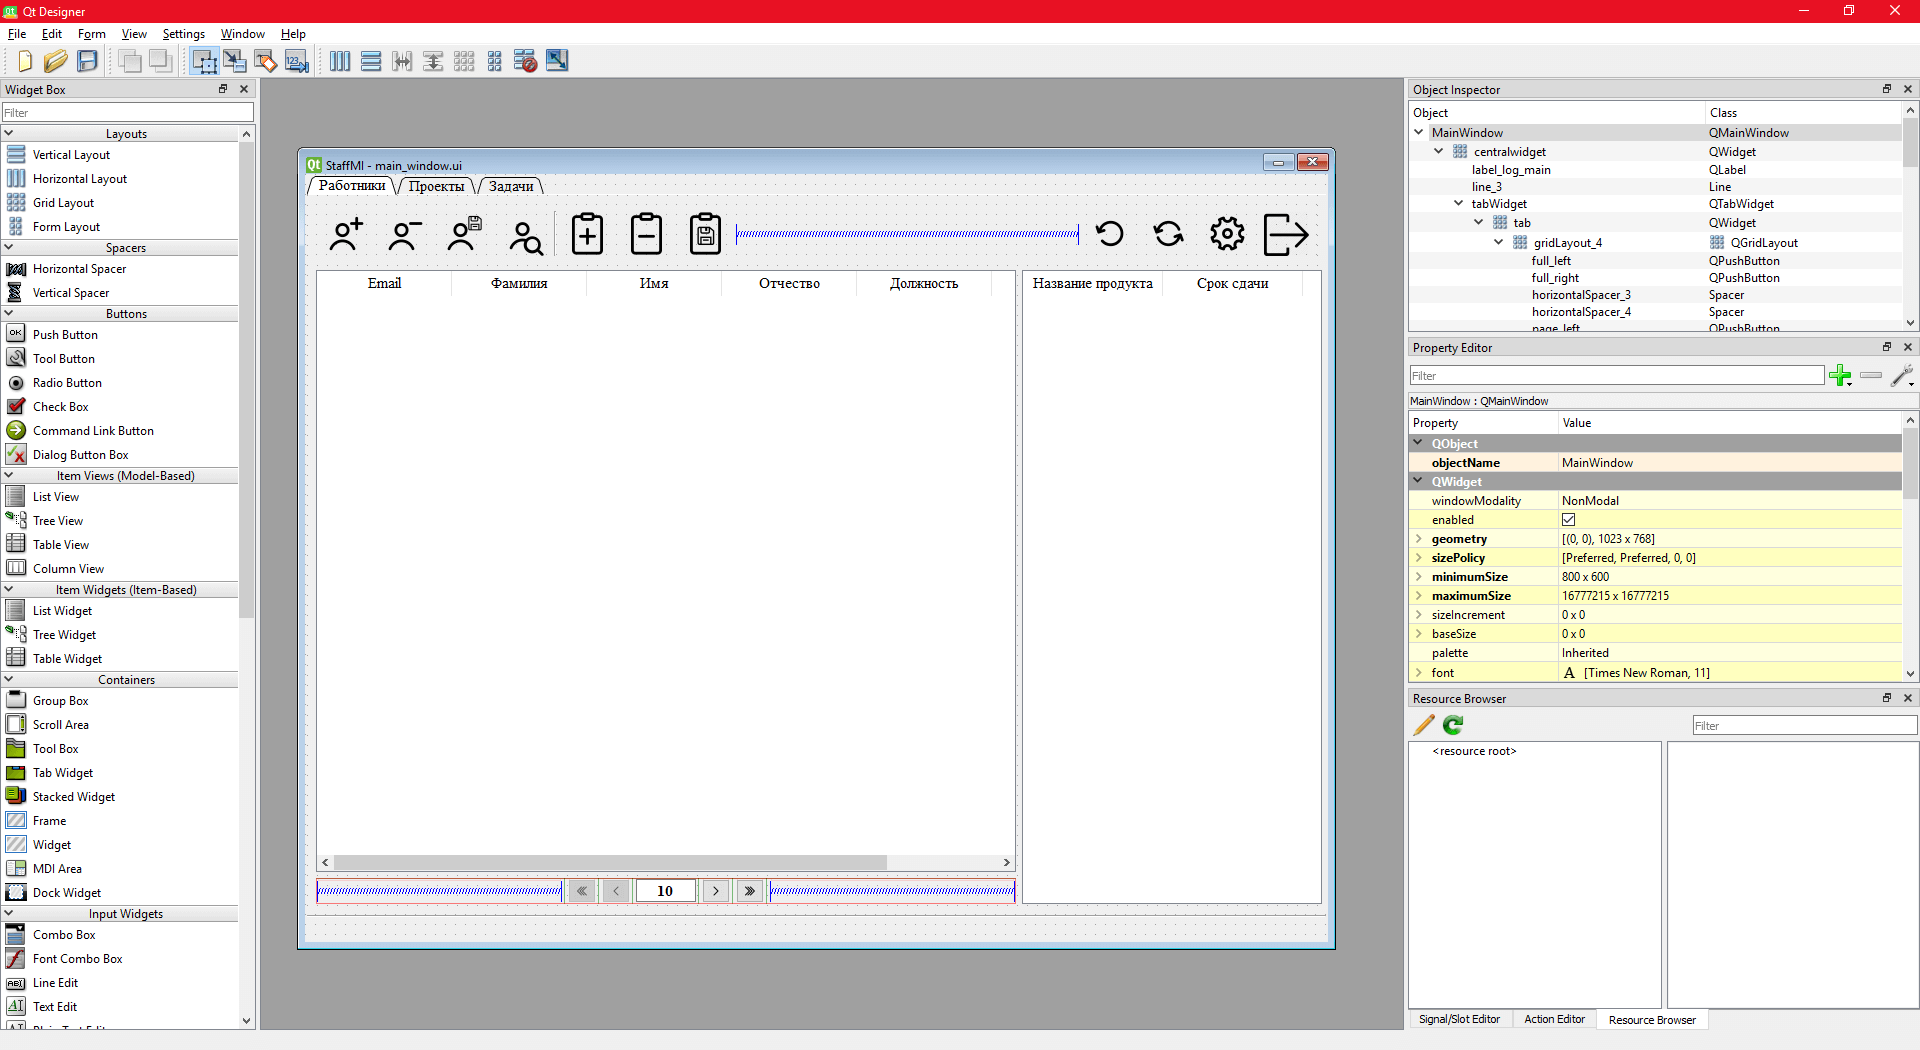
\includegraphics[width=\textwidth]{img/qtdesigner.png}\\
Рис. 7: редактирование главного меню клиента в Qt Designer.\\[\baselineskip]
\end{center}


\newpage
\subsection{Реализация}
Основная логика работы и обработки событий в интерфейсе клиента реализована за счет языка программирования Python. Для обращения серверу используется собственное API. Для обработки json файлов используется библиотека json. Для работы с Qt5 используется библиотека PyQt5 и ее производные (QtWidgets, QtCore, QtGui и т.д.). Для работы с post-запросами используется библиотека requests.

В файле db\_api.py реализована работа собственного API. Он представляет список функций-запросов к серверу, которые вызываются по мере необходимости.
\begin{center}
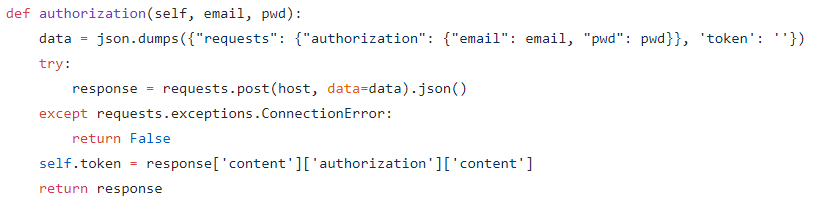
\includegraphics[scale=0.7]{img/authorization_client.png}\\
Рис. 8: функция авторизации клиента.\\[\baselineskip]
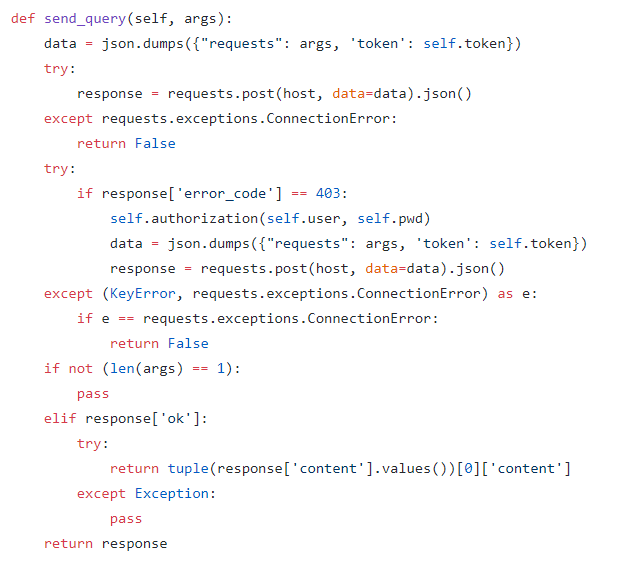
\includegraphics[scale=0.6]{img/send_query.png}\\
Рис. 9: функция отправки запроса на сервер и последующей обработки ответа.\\[\baselineskip]
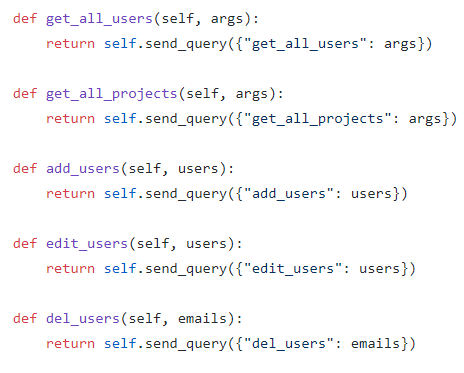
\includegraphics[scale=0.7]{img/other_func.png}\\
Рис. 10: примеры функций-запросов.\\[\baselineskip]
\end{center}

В файле main\_logic.py реализована вся логика работы интерфейса. Различные нажатия, события и процессы обрабатывается по средствам методов того класса, к которому они относятся. Разделение по классам необходима для реализации многооконного интерфейса. Каждый такой класс имеет свои методы для обработки различных действий и событий. В данный момент таких классов 5, а именно:
\begin{itemize}
  \item miWindow – класс, отвечающий за главное окно интерфейса.
  \item loginStackWindow – класс, отвечающий за окно авторизации и смены пароля пользователя.
  \item inprojectDialogWindow – класс, отвечающий за диалог добавления работника в проект.
  \item newProjectDialogWindow – класс, отвечающий за диалог создания нового проекта.
  \item newUserDialogWindow – класс, отвечающий за диалог добавления нового пользователя.
\end{itemize}

Главенствующим классом считается miWindow, он же и самый объемный. Несмотря на это, первым делом, пользователь увидит окно авторизации, за которое отвечает класс loginStackWindow, в котором и будет создан объект главного класса.


\newpage
\subsection{Принципы работы клиента}
После запуска приложения, пользователь увидит окно авторизации. В нем же он может изменить пароль от своей учетной записи. После успешного прохождения этапа аутентификации, пользователь попадает на главное окно интерфейса, где доступны подменю работы с работниками и проектами.
\begin{center}
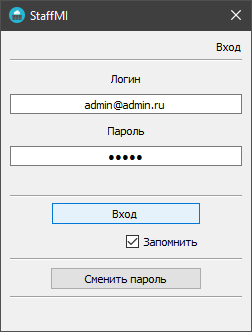
\includegraphics[scale=0.7]{img/auth_window_win.png}\\
Рис. 11: окно авторизации пользователя.\\[\baselineskip]
\end{center}

Пользователь может отредактировать данные любого проекта или работника, добавить новых, связать выбранных работников с проектом, а также удалять любые проекты и любых работников. Все изменения данных будут отображены специальными цветами:
\begin{itemize}
  \item Зеленый – добавленная запись;
  \item Желтый – отредактированная запись;
  \item Красный – удаленная запись.
\end{itemize}

\begin{center}
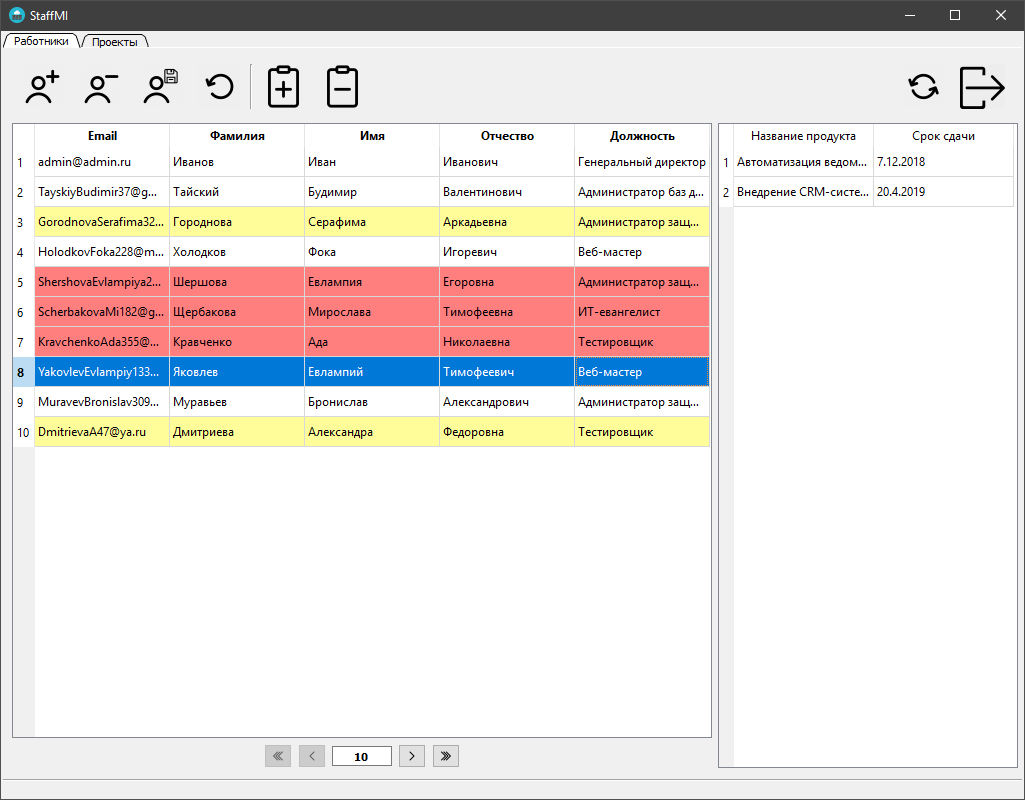
\includegraphics[width=\textwidth]{img/main_window_win.png}\\
Рис. 12: главное окно интерфейса.\\[\baselineskip]
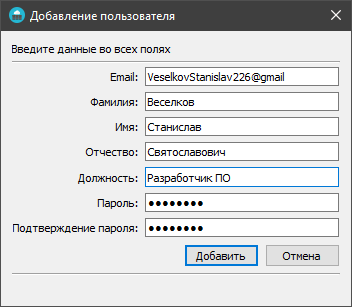
\includegraphics[scale=0.6]{img/add_user_window_win.png}\\
Рис. 13: окно добавления нового пользователя.\\[\baselineskip]
\end{center}

Все данные, которые были изменены пользователем, будут хранится во временной памяти до тех пор, пока не будет дана команда отправки изменений на сервер. Сделанные изменения можно отменить, если они еще не были отправлены на сервер. Для предотвращения переизбытка используемой оперативной памяти используется постраничное отображение информации.

Размер этих страниц можно настроить. В режиме реального времени происходит проверка соединения с сервером. Если произойдет разрыв соединения, пользователь будет предупрежден, а функционал интерфейса урезан. Обновление истекшего токена происходит во время работы программы так, что бы пользователь не замечал этого – повторный ввод логина и пароля требоваться не будет.

За счет кроссплатформенности PyQt5, интерфейс клиента на других ОС не будет отличатся от интерфейса на ОС Windows 10.
\begin{center}
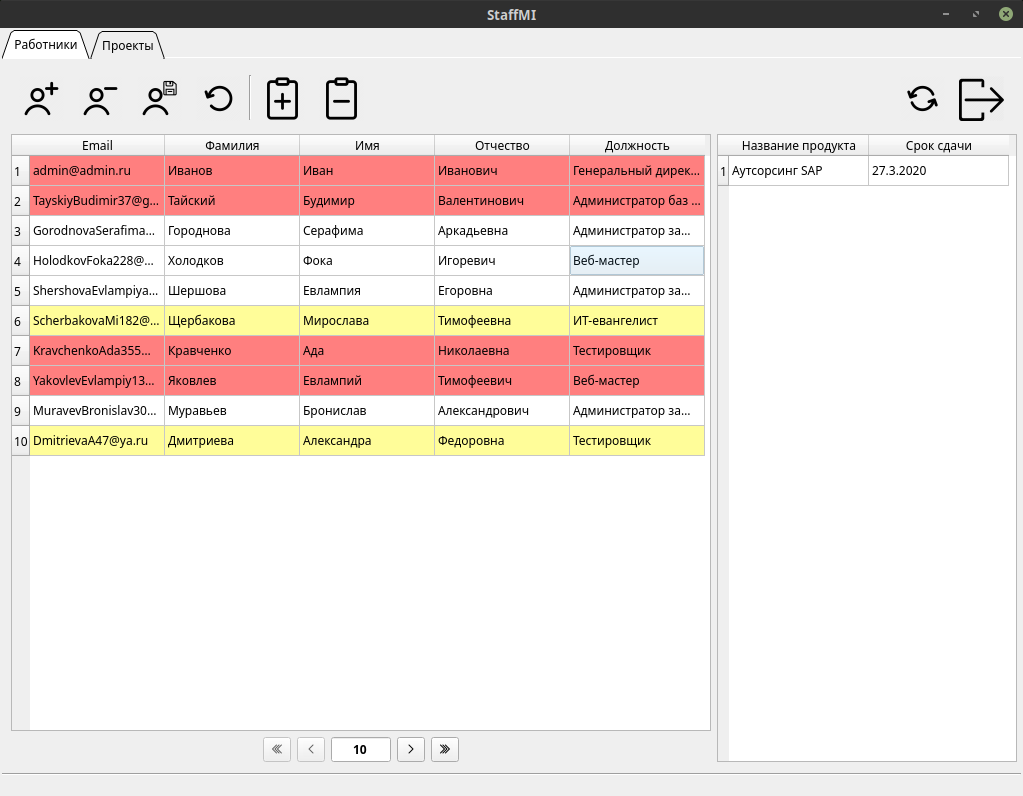
\includegraphics[width=\textwidth]{img/main_window_linux.png}\\
Рис. 14: главное окно интерфейса на ОС Linux Mint.\\[\baselineskip]
\end{center}


\newpage
\section{Заключение}
Современные технологии программирования предоставляют разработчикам неограниченные возможности для реализации своих идей. В данной дипломной работе с помощью перечисленных выше технологий было разработано клиент-серверное приложение для управления персоналом и проектами, которое дало огромный толчок в понимании клиент-серверных архитектур, а также позволило получить практический опыт разработки подобных решений.


\newpage
\section{Приложение}
\subsection{Исходный код server/app.py}
\lstinputlisting[language=Python, breaklines]{code/app.py}


\newpage
\subsection{Исходный код server/db.py}
\lstinputlisting[language=Python, breaklines]{code/db.py}


% \newpage
% \subsection{Исходный код server/tests.py}
% \lstinputlisting[language=Python, breaklines]{code/tests.py}


\newpage
\subsection{Исходный код client/db\_api.py}
\lstinputlisting[language=Python, breaklines]{code/db_api.py}


\newpage
\subsection{Исходный код client/main\_logic.py}
\lstinputlisting[language=Python, breaklines]{code/main_logic.py}


\newpage
\addcontentsline{toc}{section}{Список литературы}
\begin{thebibliography}{}
\bibitem{}
Документация Qt5 [Электронный ресурс]: для версии 5.12. URL: https://doc.qt.io/qt-5/ (дата обращения: 01.11.2018).
\bibitem{}
Документация языка програмирования Python [Электронный ресурс]: для версии 3.6. URL: https://docs.python.org/3/ (дата обращения: 10.10.2018).
\bibitem{}
Шлее Макс. Qt 5.10. Профессиональное программирование на C++. --- Санкт-Петербург, 2018. --- 1072 с.
\bibitem{}
Марк Саммерфилд. Программирование на Python 3. Подробное руководство. --- Символ-Плюс, 2009. --- 608 с.
\end{thebibliography}

\end{document}
